       
                %% bare_jrnl.tex
%% V1.4b
%% 2015/08/26
%% by Michael Shell
%% see http://www.michaelshell.org/
%% for current contact information.
%%
%% This is a skeleton file demonstrating the use of IEEEtran.cls
%% (requires IEEEtran.cls version 1.8b or later) with an IEEE
%% journal paper.
%%
%% Support sites:
%% http://www.michaelshell.org/tex/ieeetran/
%% http://www.ctan.org/pkg/ieeetran
%% and
%% http://www.ieee.org/

%%*************************************************************************
%% Legal Notice:
%% This code is offered as-is without any warranty either expressed or
%% implied; without even the implied warranty of MERCHANTABILITY or
%% FITNESS FOR A PARTICULAR PURPOSE! 
%% User assumes all risk.
%% In no event shall the IEEE or any contributor to this code be liable for
%% any damages or losses, including, but not limited to, incidental,
%% consequential, or any other damages, resulting from the use or misuse
%% of any information contained here.
%%
%% All comments are the opinions of their respective authors and are not
%% necessarily endorsed by the IEEE.
%%
%% This work is distributed under the LaTeX Project Public License (LPPL)
%% ( http://www.latex-project.org/ ) version 1.3, and may be freely used,
%% distributed and modified. A copy of the LPPL, version 1.3, is included
%% in the base LaTeX documentation of all distributions of LaTeX released
%% 2003/12/01 or later.
%% Retain all contribution notices and credits.
%% ** Modified files should be clearly indicated as such, including  **
%% ** renaming them and changing author support contact information. **
%%*************************************************************************


% *** Authors should verify (and, if needed, correct) their LaTeX system  ***
% *** with the testflow diagnostic prior to trusting their LaTeX platform ***
% *** with production work. The IEEE's font choices and paper sizes can   ***
% *** trigger bugs that do not appear when using other class files.       ***                          ***
% The testflow support page is at:
% http://www.michaelshell.org/tex/testflow/


% Please refer to your journal's instructions for other
% options that should be set.
\documentclass[journal,onecolumn]{IEEEtran}
%
% If IEEEtran.cls has not been installed into the LaTeX system files,
% manually specify the path to it like:
% \documentclass[journal]{../sty/IEEEtran}
\usepackage[export]{adjustbox}
\usepackage{graphicx}
\usepackage{tabto}
\usepackage{placeins}
\usepackage{float}
\usepackage{hyperref}
\usepackage{algpseudocode}
\usepackage{algorithm}   

% Some very useful LaTeX packages include:
% (uncomment the ones you want to load)


% *** MISC UTILITY PACKAGES ***
%
%\usepackage{ifpdf}
% Heiko Oberdiek's ifpdf.sty is very useful if you need conditional
% compilation based on whether the output is pdf or dvi.
% usage:
% \ifpdf
%   % pdf code
% \else
%   % dvi code
% \fi
% The latest version of ifpdf.sty can be obtained from:
% http://www.ctan.org/pkg/ifpdf
% Also, note that IEEEtran.cls V1.7 and later provides a builtin
% \ifCLASSINFOpdf conditional that works the same way.
% When switching from latex to pdflatex and vice-versa, the compiler may
% have to be run twice to clear warning/error messages.






% *** CITATION PACKAGES ***
%
%\usepackage{cite}
% cite.sty was written by Donald Arseneau
% V1.6 and later of IEEEtran pre-defines the format of the cite.sty package
% \cite{} output to follow that of the IEEE. Loading the cite package will
% result in citation numbers being automatically sorted and properly
% "compressed/ranged". e.g., [1], [9], [2], [7], [5], [6] without using
% cite.sty will become [1], [2], [5]--[7], [9] using cite.sty. cite.sty's
% \cite will automatically add leading space, if needed. Use cite.sty's
% noadjust option (cite.sty V3.8 and later) if you want to turn this off
% such as if a citation ever needs to be enclosed in parenthesis.
% cite.sty is already installed on most LaTeX systems. Be sure and use
% version 5.0 (2009-03-20) and later if using hyperref.sty.
% The latest version can be obtained at:
% http://www.ctan.org/pkg/cite
% The documentation is contained in the cite.sty file itself.






% *** GRAPHICS RELATED PACKAGES ***
%
\ifCLASSINFOpdf
  % \usepackage[pdftex]{graphicx}
  % declare the path(s) where your graphic files are
  % \graphicspath{{../pdf/}{../jpeg/}}
  % and their extensions so you won't have to specify these with
  % every instance of \includegraphics
  % \DeclareGraphicsExtensions{.pdf,.jpeg,.png}
\else
  % or other class option (dvipsone, dvipdf, if not using dvips). graphicx
  % will default to the driver specified in the system graphics.cfg if no
  % driver is specified.
  % \usepackage[dvips]{graphicx}
  % declare the path(s) where your graphic files are
  % \graphicspath{{../eps/}}
  % and their extensions so you won't have to specify these with
  % every instance of \includegraphics
  % \DeclareGraphicsExtensions{.eps}
\fi
% graphicx was written by David Carlisle and Sebastian Rahtz. It is
% required if you want graphics, photos, etc. graphicx.sty is already
% installed on most LaTeX systems. The latest version and documentation
% can be obtained at: 
% http://www.ctan.org/pkg/graphicx
% Another good source of documentation is "Using Imported Graphics in
% LaTeX2e" by Keith Reckdahl which can be found at:
% http://www.ctan.org/pkg/epslatex
%
% latex, and pdflatex in dvi mode, support graphics in encapsulated
% postscript (.eps) format. pdflatex in pdf mode supports graphics
% in .pdf, .jpeg, .png and .mps (metapost) formats. Users should ensure
% that all non-photo figures use a vector format (.eps, .pdf, .mps) and
% not a bitmapped formats (.jpeg, .png). The IEEE frowns on bitmapped formats
% which can result in "jaggedy"/blurry rendering of lines and letters as
% well as large increases in file sizes.
%
% You can find documentation about the pdfTeX application at:
% http://www.tug.org/applications/pdftex





% *** MATH PACKAGES ***
%
%\usepackage{amsmath}
% A popular package from the American Mathematical Society that provides
% many useful and powerful commands for dealing with mathematics.
%
% Note that the amsmath package sets \interdisplaylinepenalty to 10000
% thus preventing page breaks from occurring within multiline equations. Use:
%\interdisplaylinepenalty=2500
% after loading amsmath to restore such page breaks as IEEEtran.cls normally
% does. amsmath.sty is already installed on most LaTeX systems. The latest
% version and documentation can be obtained at:
% http://www.ctan.org/pkg/amsmath





% *** SPECIALIZED LIST PACKAGES ***
%
%\usepackage{algorithmic}
% algorithmic.sty was written by Peter Williams and Rogerio Brito.
% This package provides an algorithmic environment fo describing algorithms.
% You can use the algorithmic environment in-text or within a figure
% environment to provide for a floating algorithm. Do NOT use the algorithm
% floating environment provided by algorithm.sty (by the same authors) or
% algorithm2e.sty (by Christophe Fiorio) as the IEEE does not use dedicated
% algorithm float types and packages that provide these will not provide
% correct IEEE style captions. The latest version and documentation of
% algorithmic.sty can be obtained at:
% http://www.ctan.org/pkg/algorithms
% Also of interest may be the (relatively newer and more customizable)
% algorithmicx.sty package by Szasz Janos:
% http://www.ctan.org/pkg/algorithmicx




% *** ALIGNMENT PACKAGES ***
%
%\usepackage{array}
% Frank Mittelbach's and David Carlisle's array.sty patches and improves
% the standard LaTeX2e array and tabular environments to provide better
% appearance and additional user controls. As the default LaTeX2e table
% generation code is lacking to the point of almost being broken with
% respect to the quality of the end results, all users are strongly
% advised to use an enhanced (at the very least that provided by array.sty)
% set of table tools. array.sty is already installed on most systems. The
% latest version and documentation can be obtained at:
% http://www.ctan.org/pkg/array


% IEEEtran contains the IEEEeqnarray family of commands that can be used to
% generate multiline equations as well as matrices, tables, etc., of high
% quality.




% *** SUBFIGURE PACKAGES ***
%\ifCLASSOPTIONcompsoc
%  \usepackage[caption=false,font=normalsize,labelfont=sf,textfont=sf]{subfig}
%\else
%  \usepackage[caption=false,font=footnotesize]{subfig}
%\fi
% subfig.sty, written by Steven Douglas Cochran, is the modern replacement
% for subfigure.sty, the latter of which is no longer maintained and is
% incompatible with some LaTeX packages including fixltx2e. However,
% subfig.sty requires and automatically loads Axel Sommerfeldt's caption.sty
% which will override IEEEtran.cls' handling of captions and this will result
% in non-IEEE style figure/table captions. To prevent this problem, be sure
% and invoke subfig.sty's "caption=false" package option (available since
% subfig.sty version 1.3, 2005/06/28) as this is will preserve IEEEtran.cls
% handling of captions.
% Note that the Computer Society format requires a larger sans serif font
% than the serif footnote size font used in traditional IEEE formatting
% and thus the need to invoke different subfig.sty package options depending
% on whether compsoc mode has been enabled.
%
% The latest version and documentation of subfig.sty can be obtained at:
% http://www.ctan.org/pkg/subfig




% *** FLOAT PACKAGES ***
%
%\usepackage{fixltx2e}
% fixltx2e, the successor to the earlier fix2col.sty, was written by
% Frank Mittelbach and David Carlisle. This package corrects a few problems
% in the LaTeX2e kernel, the most notable of which is that in current
% LaTeX2e releases, the ordering of single and double column floats is not
% guaranteed to be preserved. Thus, an unpatched LaTeX2e can allow a
% single column figure to be placed prior to an earlier double column
% figure.
% Be aware that LaTeX2e kernels dated 2015 and later have fixltx2e.sty's
% corrections already built into the system in which case a warning will
% be issued if an attempt is made to load fixltx2e.sty as it is no longer
% needed.
% The latest version and documentation can be found at:
% http://www.ctan.org/pkg/fixltx2e


%\usepackage{stfloats}
% stfloats.sty was written by Sigitas Tolusis. This package gives LaTeX2e
% the ability to do double column floats at the bottom of the page as well
% as the top. (e.g., "\begin{figure*}[!b]" is not normally possible in
% LaTeX2e). It also provides a command:
%\fnbelowfloat
% to enable the placement of footnotes below bottom floats (the standard
% LaTeX2e kernel puts them above bottom floats). This is an invasive package
% which rewrites many portions of the LaTeX2e float routines. It may not work
% with other packages that modify the LaTeX2e float routines. The latest
% version and documentation can be obtained at:
% http://www.ctan.org/pkg/stfloats
% Do not use the stfloats baselinefloat ability as the IEEE does not allow
% \baselineskip to stretch. Authors submitting work to the IEEE should note
% that the IEEE rarely uses double column equations and that authors should try
% to avoid such use. Do not be tempted to use the cuted.sty or midfloat.sty
% packages (also by Sigitas Tolusis) as the IEEE does not format its papers in
% such ways.
% Do not attempt to use stfloats with fixltx2e as they are incompatible.
% Instead, use Morten Hogholm'a dblfloatfix which combines the features
% of both fixltx2e and stfloats:
%
% \usepackage{dblfloatfix}
% The latest version can be found at:
% http://www.ctan.org/pkg/dblfloatfix




%\ifCLASSOPTIONcaptionsoff
%  \usepackage[nomarkers]{endfloat}
% \let\MYoriglatexcaption\caption
% \renewcommand{\caption}[2][\relax]{\MYoriglatexcaption[#2]{#2}}
%\fi
% endfloat.sty was written by James Darrell McCauley, Jeff Goldberg and 
% Axel Sommerfeldt. This package may be useful when used in conjunction with 
% IEEEtran.cls'  captionsoff option. Some IEEE journals/societies require that
% submissions have lists of figures/tables at the end of the paper and that
% figures/tables without any captions are placed on a page by themselves at
% the end of the document. If needed, the draftcls IEEEtran class option or
% \CLASSINPUTbaselinestretch interface can be used to increase the line
% spacing as well. Be sure and use the nomarkers option of endfloat to
% prevent endfloat from "marking" where the figures would have been placed
% in the text. The two hack lines of code above are a slight modification of
% that suggested by in the endfloat docs (section 8.4.1) to ensure that
% the full captions always appear in the list of figures/tables - even if
% the user used the short optional argument of \caption[]{}.
% IEEE papers do not typically make use of \caption[]'s optional argument,
% so this should not be an issue. A similar trick can be used to disable
% captions of packages such as subfig.sty that lack options to turn off
% the subcaptions:
% For subfig.sty:
% \let\MYorigsubfloat\subfloat
% \renewcommand{\subfloat}[2][\relax]{\MYorigsubfloat[]{#2}}
% However, the above trick will not work if both optional arguments of
% the \subfloat command are used. Furthermore, there needs to be a
% description of each subfigure *somewhere* and endfloat does not add
% subfigure captions to its list of figures. Thus, the best approach is to
% avoid the use of subfigure captions (many IEEE journals avoid them anyway)
% and instead reference/explain all the subfigures within the main caption.
% The latest version of endfloat.sty and its documentation can obtained at:
% http://www.ctan.org/pkg/endfloat
%
% The IEEEtran \ifCLASSOPTIONcaptionsoff conditional can also be used
% later in the document, say, to conditionally put the References on a 
% page by themselves.




% *** PDF, URL AND HYPERLINK PACKAGES ***
%
%\usepackage{url}
% url.sty was written by Donald Arseneau. It provides better support for
% handling and breaking URLs. url.sty is already installed on most LaTeX
% systems. The latest version and documentation can be obtained at:
% http://www.ctan.org/pkg/url
% Basically, \url{my_url_here}.




% *** Do not adjust lengths that control margins, column widths, etc. ***
% *** Do not use packages that alter fonts (such as pslatex).         ***
% There should be no need to do such things with IEEEtran.cls V1.6 and later.
% (Unless specifically asked to do so by the journal or conference you plan
% to submit to, of course. )


% correct bad hyphenation here
\hyphenation{op-tical net-works semi-conduc-tor}


\begin{document}
%
% paper title
% Titles are generally capitalized except for words such as a, an, and, as,
% at, but, by, for, in, nor, of, on, or, the, to and up, which are usually
% not capitalized unless they are the first or last word of the title.
% Linebreaks \\ can be used within to get better formatting as desired.
% Do not put math or special symbols in the title.
\title{Laboratorio Closest Pair con LinkedList}
%
%
% author names and IEEE memberships
% note positions of commas and nonbreaking spaces ( ~ ) LaTeX will not break
% a structure at a ~ so this keeps an author's name from being broken across
% two lines.
% use \thanks{} to gain access to the first footnote area
% a separate \thanks must be used for each paragraph as LaTeX2e's \thanks
% was not built to handle multiple paragraphs
%

\author{Alan~Daniel~Florez~Cerro,~\IEEEmembership{~Ingenieria de sistemas}}

% note the % following the last \IEEEmembership and also \thanks - 
% these prevent an unwanted space from occurring between the last author name
% and the end of the author line. i.e., if you had this:
% 
% \author{....lastname \thanks{...} \thanks{...} }
%                     ^------------^------------^----Do not want these spaces!
%
% a space would be appended to the last name and could cause every name on that
% line to be shifted left slightly. This is one of those "LaTeX things". For
% instance, "\textbf{A} \textbf{B}" will typeset as "A B" not "AB". To get
% "AB" then you have to do: "\textbf{A}\textbf{B}"
% \thanks is no different in this regard, so shield the last } of each \thanks
% that ends a line with a % and do not let a space in before the next \thanks.
% Spaces after \IEEEmembership other than the last one are OK (and needed) as
% you are supposed to have spaces between the names. For what it is worth,
% this is a minor point as most people would not even notice if the said evil
% space somehow managed to creep in.



% The paper headers
\markboth{Uninorte, Noviembre~2022}%
{Shell \MakeLowercase{\textit{et al.}}: Bare Demo of IEEEtran.cls for IEEE Journals}
% The only time the second header will appear is for the odd numbered pages
% after the title page when using the twoside option.
% 
% *** Note that you probably will NOT want to include the author's ***
% *** name in the headers of peer review papers.                   ***
% You can use \ifCLASSOPTIONpeerreview for conditional compilation here if
% you desire.




% If you want to put a publisher's ID mark on the page you can do it like
% this:
%\IEEEpubid{0000--0000/00\$00.00~\copyright~2015 IEEE}
% Remember, if you use this you must call \IEEEpubidadjcol in the second
% column for its text to clear the IEEEpubid mark.


% use for special paper notices
%\IEEEspecialpapernotice{(Invited Paper)}


% make the title area
\maketitle

% As a general rule, do not put math, special symbols or citations
% in the abstract or keywords.

\begin{abstract}
El siguiente laboratorio se enfoca, como en el laboratorio anterior, en analizar el comportamiento de un algoritmo que compara las distancias de un conjunto de puntos generados aleatoriamente y determina que par de puntos es el más cercano.  Sin embargo, esta vez la estructura de datos usada para las pruebas será una implementación propia de listas enlazadas.
Igual que en el laboratorio anterior, se determinará el par más cercano usando las estrategias de fuerza bruta y "divide and conquer"), observando el tiempo de ejecución de cada una en distintos conjuntos de puntos aleatorios, donde la mitad tendrá un x menor a cierto valor y la otra mitad tendrá un x mayor a dicho valor. Se reutilizará gran parte de la implementación en java anterior y de los resultados obtenidos vemos que usando listas enlazadas como estructura de datos causa que el tiempo de ejecución de los algoritmos crezca en comparación a usar ArryList
\end{abstract}

% Note that keywords are not normally used for peerreview papers.
\begin{IEEEkeywords}
divide and conquer, fuerza bruta. complejidad, LinkedList.
\end{IEEEkeywords}

% For peer review papers, you can put extra information on the cover
% page as needed:
% \ifCLASSOPTIONpeerreview
% \begin{center} \bfseries EDICS Category: 3-BBND \end{center}
% \fi
%
% For peerreview papers, this IEEEtran command inserts a page break and
% creates the second title. It will be ignored for other modes.
\IEEEpeerreviewmaketitle


\section{Introducción}
% The very first letter is a 2 line initial drop letter followed
% by the rest of the first word in caps.
% 
% form to use if the first word consists of a single letter:
% \IEEEPARstart{A}{demo} file is ....
% 
% form to use if you need the single drop letter followed by
% normal text (unknown if ever used by the IEEE):
% \IEEEPARstart{A}{}demo file is ....
% 
% Some journals put the first two words in caps:
% \IEEEPARstart{T}{his demo} file is ....
% 
% Here we have the typical use of a "T" for an initial drop letter
% and "HIS" in caps to complete the first word.
\IEEEPARstart{E}{l} objetivo principal de este informe es determinar si los resultados para la complejidad de ambas estrategias se ve alterado de alguna manera al utilizar una estructura de datos (LinkedList implementada por uno mismo), poniéndolas a prueba con distintos casos para así poder elaborar una gráfica con los resultados obtenidos de los tiempos de ejecución que ilustre la complejidad de cada una.\\

Esto es importante porque permite ver como el uso de una estructura de datos distinta puede alterar los resultados previamente obtenidos. Además, podemos esperar que el numero de iteraciones no se vea muy afectado pero si los tiempos de ejecución pues el usar listas enlazadas no cambia las iteraciones que requiere realizar el algoritmo para calcular el par más cercano, lo que nos permite obtener una nueva perspectiva respecto al informe anterior, cuyos resultados se usarán para comparación.\\

Es importante resaltar que se hace uso de listas enlazadas pues, como menciona Cairó(2006):\\
\begin{quote}
Este es un tipo de estructura lineal y dinámica de datos. Lineal porque a cada elemento le puede seguir sólo otro elemento; dinámica) porque se puede manejar la memoria de manera flexible, sin necesidad de reservar espacio con antelación.
La principal ventaja de manejar un tipo dinámico de datos es que se pueden adquirir posiciones de memoria a medida que se necesitan; éstas se liberan cuando ya no se requieren.    
\end{quote}



\hfill mds
 
\hfill Noviembre 24, 2022

\input{sections/definición de problema.tex}

\section{Metodología}
Se tomará el tiempo de ejecución del algoritmo de fuerza bruta y de "divide y vencerás" usando una implemenatción propia de listas enlazadas y usando ArrayLists en conjuntos de n puntos generados aleatoriamente y ordenados de forma ascendente respecto a su valor de x donde n aumentará en potencias de 2 desde $2^2$ hasta que el tiempo de ejecución sea demasiado alto, en caso de la versión con ArrayList se logró ejecutar hasta con $2^{18}$ puntos y en el caso de la versión con LinkedList hasta  $2^{14}$ puntos.\\

\textbf{Nota:} La implementación de la lista enlazada personalizada se puede ver en: \url{https://github.com/adcerro/closest_linked-list_/blob/main/LinkedList.java}

Para el algoritmo de fuerza bruta se tomará el tiempo y las iteraciones obtenidas un vez ejecutado sobre el conjunto de puntos, por otra parte para el algoritmo de divide y vencerás se ejecutara el mismo cuatro veces sobre conjuntos aleatorios distintos para cada tamaño n y los tiempos e iteraciones obtenidas serán promediados.\\

El tiempo en nanosegundos se medirá usando la función System.nanotime() de java antes y después de las lineas de código que llaman a cada algoritmo, la resta de ambas permite hallar el tiempo de ejecución del algoritmo.

Para contar las  iteraciones se pondrá un contador dentro de los ciclos usados para determinar el par de puntos más cercanos. A continuación se muestran los algoritmos usados:

\begin{algorithm}[h!]
\caption{Algoritmo de fuerza bruta}
\begin{algorithmic}
\State $bruteForce(list)$
    \State $closest[] \gets Empty$
    \State $closest[0] \gets distance(list[0], list[1])$
    \State $closest[1] \gets list[0].x$
    \State $closest[2] \gets list[0].y$
    \State $closest[3] \gets list[1].x$
    \State $closest[4] \gets list[1].y$
    \For{$\texttt{j from 0 to lenght(list)-2 with increments of 1}$}
        \For{$\texttt{i from 0 to lenght(list)-1 with increments of 1}$}
        \If{$distance(list[j],list[i]) < closest[0] $} 
            \State $closest[0] \gets distance(list[j], list[i])$
            \State $ closest[1] \gets list[j].x$
            \State $ closest[2] \gets list[j].y$
            \State $ closest[3] \gets list[i].x$
            \State $ closest[4] \gets list[i].y$
        \EndIf
        \EndFor
        \State $ iterations \gets iterations + 1$
    \EndFor
\end{algorithmic}    
\end{algorithm}
\textbf{Nota:} distance(a, b) recibe dos puntos (a y b) y calcula su distancia al cuadrado usando la formula de $d^2 =(Y_2-Y_1)^2+(X_2-X1)^2$\\

El algoritmo de divide y vencerás maneja dos casos. Estos son:
\begin{itemize}
    \item 
    Los puntos más cercanos del conjunto se encuentran en el mismo subconjunto.
    \item
    Los puntos más cercanos del conjunto se encuentran cada uno en un subconjunto distinto.
\end{itemize}
Si se da el primer caso, el algoritmo anterior simplemente encuentra el par mas cercano al comparar el par de un grupo con el otro y escoger el menor.\\

Cuando se da el segundo caso se deben revisar los puntos cercanos a donde se realizó la división del grupo de puntos para poder determinar correctamente el par de puntos más cercanos. Para ello se usa una versión que sigue la misma lógica del algoritmo de fuerza bruta, solo que un tanto modificada.\\
\begin{algorithm}[h!]
\caption{Algoritmo divide y vencerás}
\begin{algorithmic}
\State $divideAndConquer(list)$
    \State $ firsthalf[] \gets \texttt{the first half of the points in the list}$
    \State $ secondhalf[] \gets \texttt{the second half of the points in the list}$
    \If{$list.size()>6$}
    \State $ f[] \gets \texttt{divideAndConquer(firsthalf)}$
    \State $ s[] \gets \texttt{divideAndConquer(secondhalf)}$
    \If{$f[0]>s[0]$}
    \State $bruteForce(firsthalf, secondhalf, s)$
    \State$\texttt{return s}$
    \Else
    \State $bruteForce(firsthalf, secondhalf, f)$
    \State$\texttt{return f}$
    \EndIf
    \Else
     \State $ first[] \gets bruteForce(firsthalf)$
    \State $ second[] \gets bruteForce(secondhalf)$
    \If{$first[0]>second[0]$}
        \State $bruteforce(firsthalf, secondhalf,second)$
        \State $\texttt{return second}$
    \Else
        \If{$first[0]=second[0]$}
            \State $bruteforce(firsthalf, secondhalf,second)$
            \State $\texttt{return second}$
        \Else
            \State $bruteforce(firsthalf, secondhalf,first)$
            \State $\texttt{return first}$
         \EndIf
    \EndIf
\EndIf
\end{algorithmic}    
\end{algorithm}

\begin{algorithm}[h!]
\caption{Algoritmo de fuerza bruta (modificado)}
\begin{algorithmic}
\State $bruteForce(listA, listB, dist[])$
    \State $firstgroup[] \gets discard(listA,lenght(listA)-1,dist[0])$
    \State $secondgroup[] \gets discard(listB,0,dist[0])$
    \For{$\texttt{j from 0 to lenght(listA)-1 with increments of 1}$}
        \For{$\texttt{i from 0 to lenght(listB)-1 with increments of 1}$}
        \If{$distance(list[j],list[i]) < dist[0] $} 
            \State $dist[0] \gets distance(list[j], list[i])$
            \State $ dist[1] \gets list[j].x$
            \State $ dist[2] \gets list[j].y$
            \State $ dist[3] \gets list[i].x$
            \State $ dist[4] \gets list[i].y$
        \EndIf
        \EndFor
        \State $ iterations \gets iterations + 1$
    \EndFor
\end{algorithmic}    
\end{algorithm}
\FloatBarrier
\textbf{Nota: } El método discard(a, b, c) (donde a es una lista, b un índice de la misma y c un array) utilizado en el algoritmo 3 recorre la lista a y calcula la distancia en x entre cada punto y el punto en el índice b. Si la distancia es menor a la distancia c entonces añade el punto a un Array o LinkedList que retorna al final.

Esto lo hace de manera recursiva, pues al estar los puntos en orden ascendente se puede saber si se debe seguir revisando en base al resultado obtenido.\\

Estos algoritmos fueron implementados en java y se pueden ver en el siguiente repositorio de github : \url{https://github.com/adcerro/closest_linked-list_.git}

Luego de obtener los resultados en un archivo de texto se pueden generar las gráficas y tablas con los datos obtenidos.

\section{Resultados}
\begin{table}[h!]
    \centering
    \begin{tabular}{|c|c|c|}
    \hline
    Puntos & Iteraciones & Tiempo (ms)\\
    \hline
    4 & 6 & 32200\\
    \hline
    8 & 28 & 43000\\
    \hline
    16 & 120 & 89600 \\
    \hline
    32 & 496 & 394100\\
    \hline
    64 & 2016 & 676500\\
    \hline
    128 & 8128 & 1087800\\
    \hline
    256 & 32640 & 4671500\\
    \hline
    512 & 130816 & 6188600\\
    \hline
    1024 & 523776 & 11980800\\
    \hline
    2048 & 2096128 & 14932100\\
    \hline
    4096 & 8386560 & 38897300\\
    \hline
    8192 & 33550336 & 168208400\\
    \hline
    16384 & 134209536 & 783966400\\
    \hline
    32768 & 536854528 & 2206748300\\
    \hline
    65536 & 2147450880 & 9461164400 \\
    \hline
    131072 & 8589869056 & 39927323800\\
    \hline
    262144 & 34359607296 & 501522026400\\
    \hline
    \end{tabular}
    \caption{Resultados fuerza bruta con ArrayList}
    \label{tab:bruteAT}
\end{table}
\begin{figure}[h!]
    \centering
    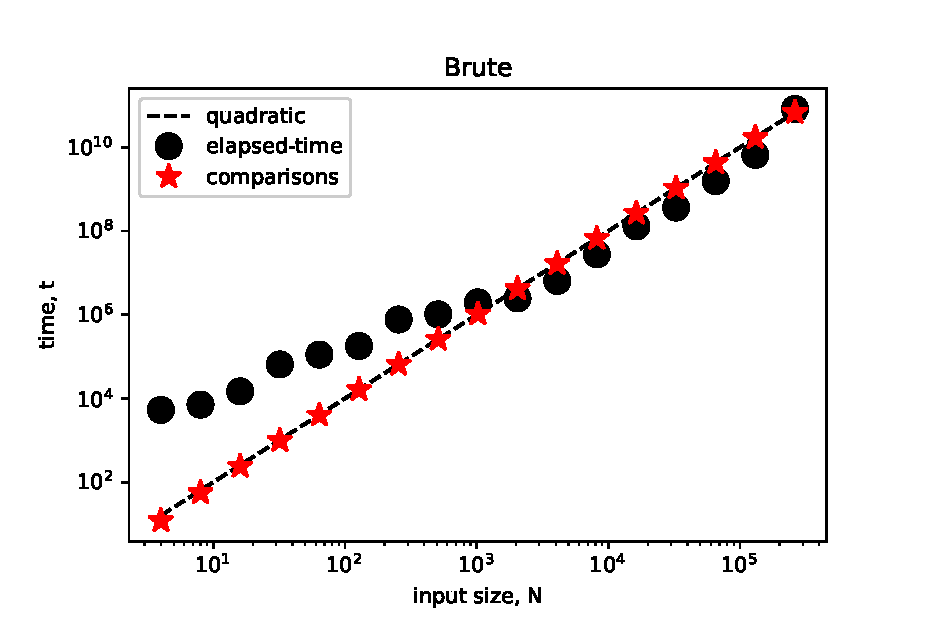
\includegraphics[scale=0.8, center]{images/bruteArrayList.eps}
    \caption{ Resultados algoritmo fuerza bruta con ArrayList}
    \label{fig:bruteAG}
\end{figure}
\begin{table}[h!]
    \centering
    \begin{tabular}{|c|c|c|}
    \hline
    Puntos & Iteraciones & Tiempo (ms)\\
    \hline
    4 & 6 & 32575\\
    \hline
    8 & 20 & 43800\\
    \hline
    16 & 40 & 7003950\\
    \hline
    32 & 57 & 87775\\
    \hline
    64 & 94 & 175200\\
    \hline
    128 & 169 & 142300\\
    \hline
    256 & 292 & 302800\\
    \hline
    512 & 488 & 235725\\
    \hline
    1024 & 884 & 451225\\
    \hline
    2048 & 1613 & 983525\\
    \hline
    4096 & 3099 & 2266750\\
    \hline
    8192 & 6187 & 4112150\\
    \hline
    16384 & 12297 & 5877875\\
    \hline
    32768 & 24528 & 9713350\\
    \hline
    65536 & 49266 & 18014550\\
    \hline
    131072 & 98349 & 47090775\\
    \hline
    262144 & 197843 & 153357475\\
    \hline
    \end{tabular}
    \caption{Resultados divide y vencerás con ArrayList}
    \label{tab:divideAT}
\end{table}
\begin{figure}[h!]
    \centering
    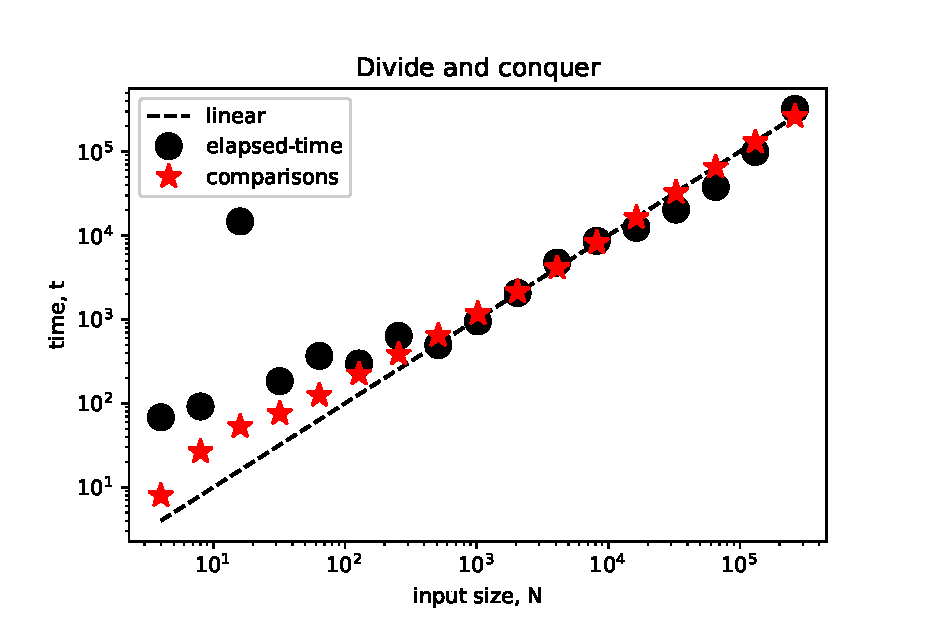
\includegraphics[scale=0.8, center]{images/divideArrayList.eps}
    \caption{Resultados algoritmo divide and conquer con ArrayList}
    \label{fig:divideAG}
\end{figure}
\FloatBarrier
\begin{table}[h!]
    \centering
    \begin{tabular}{|c|c|c|}
    \hline
    Puntos & Iteraciones & Tiempo (ms)\\
    \hline
    4 & 6 & 63700\\
    \hline
    8 & 28 & 161700\\
    \hline
    16 & 120 & 274100\\
    \hline
    32 & 496 & 667400\\
    \hline
    64 & 2016 & 6925600\\
    \hline
    128 & 8128 & 3660000\\
    \hline
    256 & 32640 & 24735900\\
    \hline
    512 & 130816 & 75925300\\
    \hline
    1024 & 523776 & 568953600\\
    \hline
    2048 & 2096128 & 4732181900\\
    \hline
    4096 & 8386560 & 39307846600\\
    \hline
    8192 & 33550336 & 322736597800\\
    \hline
    16384 & 134209536 & 4852096053400\\
    \hline
    \end{tabular}
    \caption{Resultados fuerza bruta con LinkedList}
     \label{tab:bruteLT}
\end{table}
\begin{figure}[h!]
    \centering
    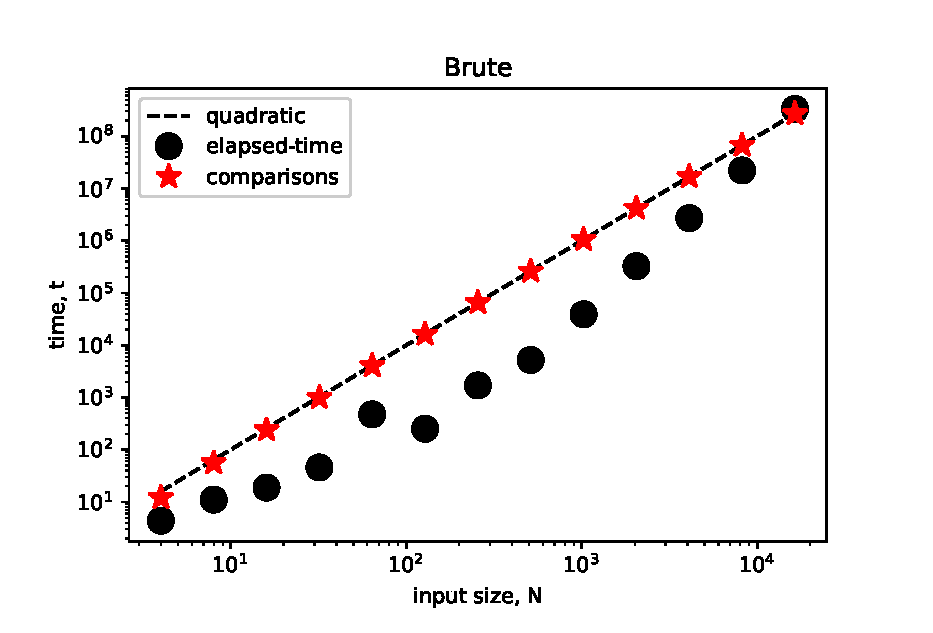
\includegraphics[scale=0.8, center]{images/bruteLinkedList.eps}
    \caption{Resultados algoritmo fuerza bruta con LinkedList}
    \label{fig:bruteLG}
\end{figure}
\FloatBarrier
\begin{table}[h!]
    \centering
    \begin{tabular}{|c|c|c|}
    \hline
    Puntos & Iteraciones & Tiempo (ms)\\
    \hline
    4 & 6 & 4446250\\
    \hline
    8 & 24 & 26500\\
    \hline
    16 & 34 & 35325\\
    \hline
    32 & 59 & 98650\\
    \hline
    64 & 103 & 225175\\
    \hline
    128 & 170 & 254675\\
    \hline
    256 & 298 & 259600\\
    \hline
    512 & 504 & 760150\\
    \hline
    1024 & 885 & 2804800\\
    \hline
    2048 & 1608 & 11440125\\
    \hline
    4096 & 3112 & 50112050\\
    \hline
    8192 & 6187 & 171533850\\
    \hline
    16384 & 12311 & 700195150\\
    \hline
    \end{tabular}
    \caption{Resultados algoritmo divide and conquer con LinkedList}
    \label{tab:divideLT}
\end{table}
\begin{figure}[h!]
    \centering
    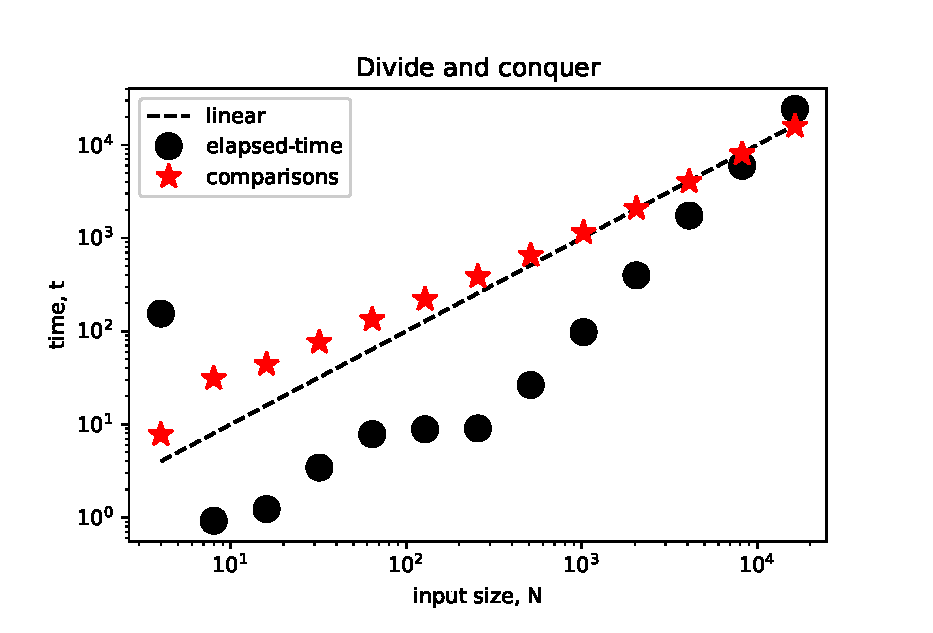
\includegraphics[scale=0.8, center]{images/divideLinkedList.eps}
    \caption{Resultados algoritmo divide and conquer con LinkedList}
    \label{fig:divideLG}
\end{figure}
\FloatBarrier

\section{Discusión}
Empezamos comparando las tablas \ref{tab:bruteAT} y \ref{tab:bruteLT}. En las mismas se observa que, como se esperaba, el número de iteraciones no se  ve alterado por el uso de ArrayList o LinkedList. También se observa con las gráficas \ref{fig:bruteAG} y \ref{fig:bruteLG} que la complejidad es la misma para ambas estructuras. Por otra parte, calculando el promedio de los tiempos de ambas usando Excel obtenemos un tiempo promedio de $4,01504*10^{11}$ ms usando LinkedList y de 32596966541 ms usando ArrayList, por lo tanto, la implementación de fuerza bruta con LinkedList consume más tiempo en promedio que la que usa ArrayList.\\

Comparando las tablas \ref{tab:divideAT} y \ref{tab:divideLT} se encuentra que el número de iteraciones ya no es igual para cada cantidad de puntos, siendo en general la implementación con LinkedList la que requiere más iteraciones para cada caso. Sin embargo, dado a que el número de iteraciones usando divide y vencerás es un promedio y la cantidad de iteraciones siempre puede variar para cada prueba, no se puede afirmar concluyentemente que el uso de LinkedList causo este aumento en las iteraciones promedio. Además, si se observan las gráficas \ref{fig:divideAG} y \ref{fig:divideLG} se nota que ambas siguen una tendencia lineal. Finalmente, calculando el promedio de los tiempos de ambas obtenemos que la implementación con LinkedList tarda en promedio 72476330,77 ms y la implementación con ArrayList tarda en promedio 14699517,65 ms, por lo tanto, la implementación de divide y vencerás con LinkedList consume más tiempo en promedio que la que usa ArrayList.\\

Una explicación para estos resultados es que la implementación personalizada de LinkedList utiliza búsqueda secuencial, lo que causa que al aumentar la cantidad de puntos se requiera una cantidad considerable de iteraciones dentro de la lista para las operaciones que requieren los algoritmos, causando el aumento en el tiempo de ejecución promedio.


% needed in second column of first page if using \IEEEpubid
%\IEEEpubidadjcol


% An example of a floating figure using the graphicx package.
% Note that \label must occur AFTER (or within) \caption.
% For figures, \caption should occur after the \includegraphics.
% Note that IEEEtran v1.7 and later has special internal code that
% is designed to preserve the operation of \label within \caption
% even when the captionsoff option is in effect. However, because
% of issues like this, it may be the safest practice to put all your
% \label just after \caption rather than within \caption{}.
%
% Reminder: the "draftcls" or "draftclsnofoot", not "draft", class
% option should be used if it is desired that the figures are to be
% displayed while in draft mode.
%
%\begin{figure}[!t]
%\centering
%\includegraphics[width=2.5in]{myfigure}
% where an .eps filename suffix will be assumed under latex, 
% and a .pdf suffix will be assumed for pdflatex; or what has been declared
% via \DeclareGraphicsExtensions.
%\caption{Simulation results for the network.}
%\label{fig_sim}
%\end{figure}

% Note that the IEEE typically puts floats only at the top, even when this
% results in a large percentage of a column being occupied by floats.


% An example of a double column floating figure using two subfigures.
% (The subfig.sty package must be loaded for this to work.)
% The subfigure \label commands are set within each subfloat command,
% and the \label for the overall figure must come after \caption.
% \hfil is used as a separator to get equal spacing.
% Watch out that the combined width of all the subfigures on a 
% line do not exceed the text width or a line break will occur.
%
%\begin{figure*}[!t]
%\centering
%\subfloat[Case I]{\includegraphics[width=2.5in]{box}%
%\label{fig_first_case}}
%\hfil
%\subfloat[Case II]{\includegraphics[width=2.5in]{box}%
%\label{fig_second_case}}
%\caption{Simulation results for the network.}
%\label{fig_sim}
%\end{figure*}
%
% Note that often IEEE papers with subfigures do not employ subfigure
% captions (using the optional argument to \subfloat[]), but instead will
% reference/describe all of them (a), (b), etc., within the main caption.
% Be aware that for subfig.sty to generate the (a), (b), etc., subfigure
% labels, the optional argument to \subfloat must be present. If a
% subcaption is not desired, just leave its contents blank,
% e.g., \subfloat[].


% An example of a floating table. Note that, for IEEE style tables, the
% \caption command should come BEFORE the table and, given that table
% captions serve much like titles, are usually capitalized except for words
% such as a, an, and, as, at, but, by, for, in, nor, of, on, or, the, to
% and up, which are usually not capitalized unless they are the first or
% last word of the caption. Table text will default to \footnotesize as
% the IEEE normally uses this smaller font for tables.
% The \label must come after \caption as always.
%
%\begin{table}[!t]
%% increase table row spacing, adjust to taste
%\renewcommand{\arraystretch}{1.3}
% if using array.sty, it might be a good idea to tweak the value of
% \extrarowheight as needed to properly center the text within the cells
%\caption{An Example of a Table}
%\label{table_example}
%\centering
%% Some packages, such as MDW tools, offer better commands for making tables
%% than the plain LaTeX2e tabular which is used here.
%\begin{tabular}{|c||c|}
%\hline
%One & Two\\
%\hline
%Three & Four\\
%\hline
%\end{tabular}
%\end{table}


% Note that the IEEE does not put floats in the very first column
% - or typically anywhere on the first page for that matter. Also,
% in-text middle ("here") positioning is typically not used, but it
% is allowed and encouraged for Computer Society conferences (but
% not Computer Society journals). Most IEEE journals/conferences use
% top floats exclusively. 
% Note that, LaTeX2e, unlike IEEE journals/conferences, places
% footnotes above bottom floats. This can be corrected via the
% \fnbelowfloat command of the stfloats package.

\section{Conclusión}
Usar una estructura de datos distinta no altera directamente las iteraciones que requiere realizar el algoritmo implementado como tal para encontrar el par de puntos más cercano. Sin embargo, la codificación/optimización de la estructura de datos si incide directamente en el tiempo de ejecución de las implementaciones y el número de iteraciones en general que realiza el programa.\\

Se puede mejorar la lista enlazada para reducir el tiempo de ejecución de las implementaciones que la utilizan empleando algoritmos de búsqueda mejor optimizados. Aún así, se debe tener en cuenta que el "manejo" de la información de listas enlazadas difiere del de ArrayList por lo que, a consideración del autor, las implementaciones de fuerza bruta y divide and conquer con listas enlazadas requieren ser pensadas e implementadas de tal forma que aprovechen eficientemente esta estructura de datos. \\

% if have a single appendix:
%\appendix[Proof of the Zonklar Equations]
% or
%\appendix  % for no appendix heading
% do not use \section anymore after \appendix, only \section*
% is possibly needed

% use appendices with more than one appendix
% then use \section to start each appendix
% you must declare a \section before using any
% \subsection or using \label (\appendices by itself
% starts a section numbered zero.)
%

% use section* for acknowledgment
\section*{Reconocimiento}
Agradecimientos al profesor Misael por su contribución a la mejora de la implementación del algoritmo para este laboratorio.

% Can use something like this to put references on a page
% by themselves when using endfloat and the captionsoff option.
\ifCLASSOPTIONcaptionsoff
  \newpage
\fi



% trigger a \newpage just before the given reference
% number - used to balance the columns on the last page
% adjust value as needed - may need to be readjusted if
% the document is modified later
%\IEEEtriggeratref{8}
% The "triggered" command can be changed if desired:
%\IEEEtriggercmd{\enlargethispage{-5in}}

% references section

% can use a bibliography generated by BibTeX as a .bbl file
% BibTeX documentation can be easily obtained at:
% http://mirror.ctan.org/biblio/bibtex/contrib/doc/
% The IEEEtran BibTeX style support page is at:
% http://www.michaelshell.org/tex/ieeetran/bibtex/
%\bibliographystyle{IEEEtran}
% argument is your BibTeX string definitions and bibliography database(s)
%\bibliography{IEEEabrv,../bib/paper}
%
% <OR> manually copy in the resultant .bbl file
% set second argument of \begin to the number of references
% (used to reserve space for the reference number labels box)

\begin{thebibliography}{1}

\bibitem{a}
Cairó, O., \& Guardati, S. (2006). Estructuras de datos. MC GRAW HILL INTERAMERICANA. Recuperado el 24 de noviembre de 2022, de  \url{http://up-rid2.up.ac.pa:8080/xmlui/handle/123456789/1299}
\bibitem{b}
Diaz Maldonado, M. (8 de Agosto de 2022). loglogPlot.py. Github. Recuperado el 26 de octubre de 2022, de \url{https://github.com/misael-diaz/computer-programming/blob/main/src/io/java/loglogPlot.py}
\bibitem{c}
How to increase the Java stack size? (13 de septiembre de 2010). Stack Overflow. Recuperado el 4 de noviembre de 2022, de  \url{https://stackoverflow.com/questions/3700459/how-to-increase-the-java-stack-size}

\end{thebibliography}


% biography section
% 
% If you have an EPS/PDF photo (graphicx package needed) extra braces are
% needed around the contents of the optional argument to biography to prevent
% the LaTeX parser from getting confused when it sees the complicated
% \includegraphics command within an optional argument. (You could create
% your own custom macro containing the \includegraphics command to make things
% simpler here.)
%\begin{IEEEbiography}[{\includegraphics[width=1in,height=1.25in,clip,keepaspectratio]{mshell}}]{Michael Shell}
% or if you just want to reserve a space for a photo:

\begin{IEEEbiography}[{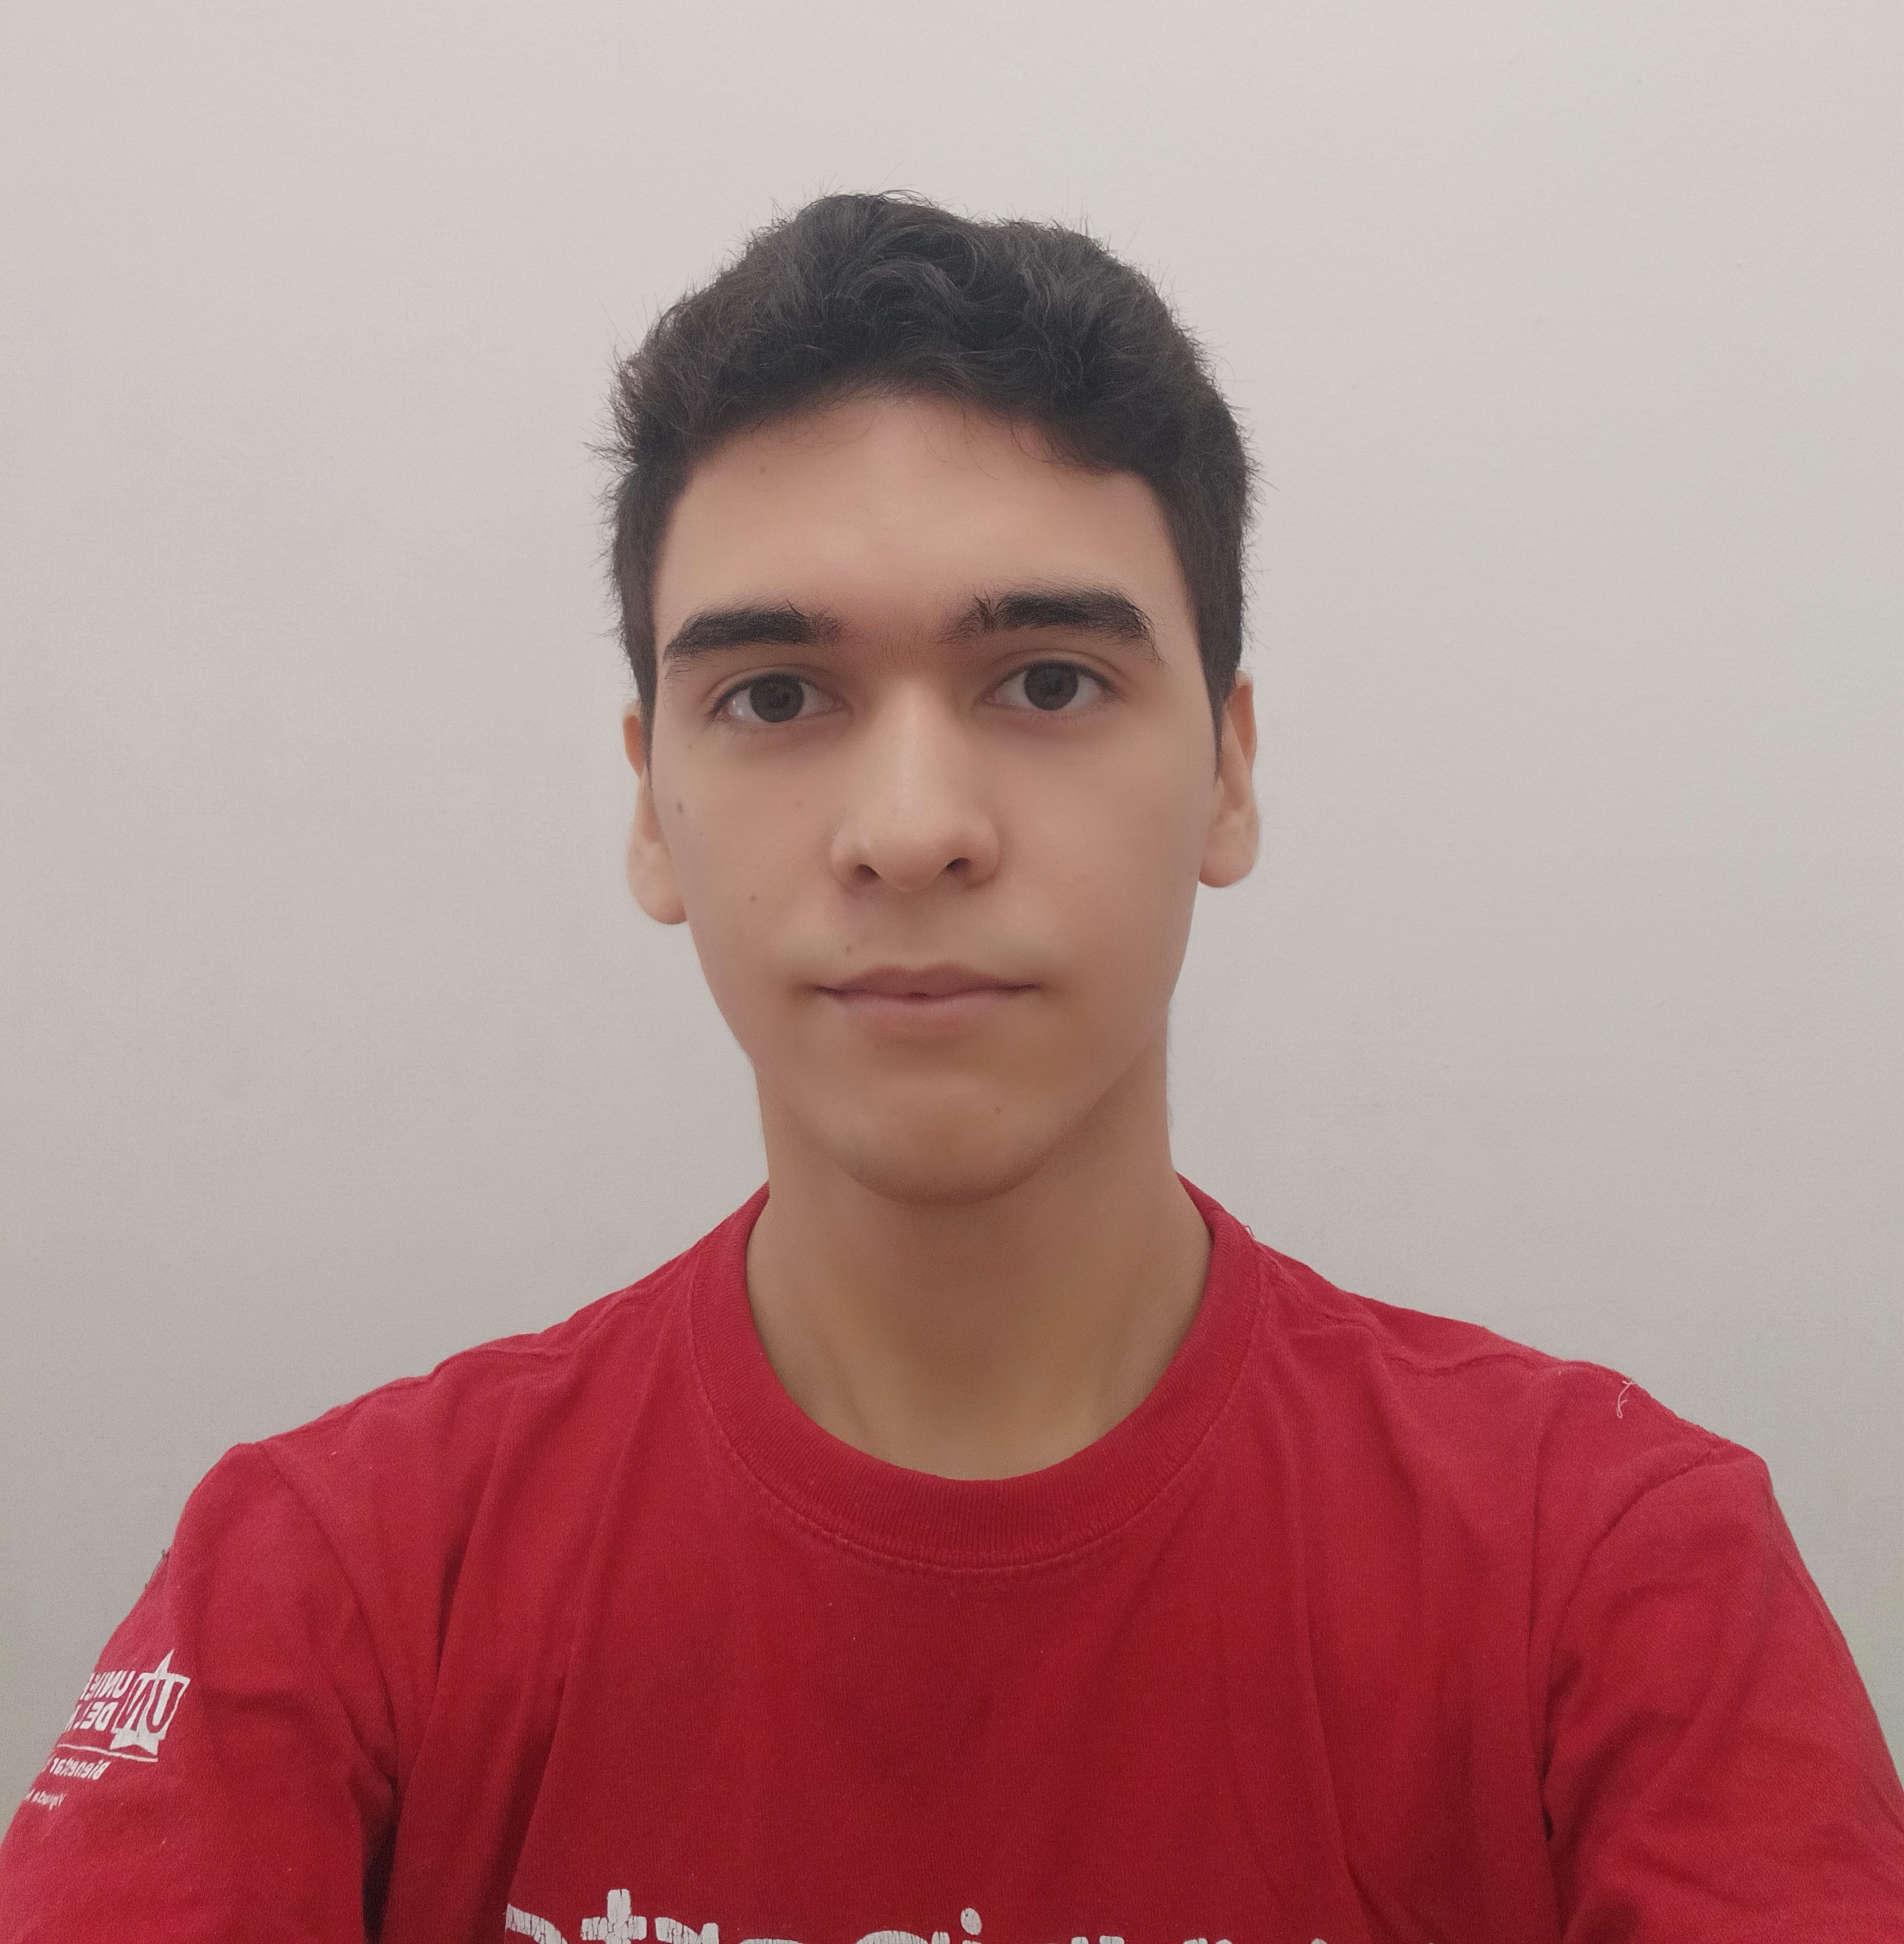
\includegraphics[width=1in,height=1.25in,clip,keepaspectratio]{images/alan.jpg}}]{Alan Florez}
Estdudiante de ingenieria de sistemas en la Universidad del norte.
\end{IEEEbiography}

% You can push biographies down or up by placing
% a \vfill before or after them. The appropriate
% use of \vfill depends on what kind of text is
% on the last page and whether or not the columns
% are being equalized.

%\vfill

% Can be used to pull up biographies so that the bottom of the last one
% is flush with the other column.
%\enlargethispage{-5in}



% that's all folks
\end{document}